\qrchapter{https://forgottenpillar.com/rsc/en-fp-chapter1}{The Foundation of Our Faith}

\egw{\textbf{The Lord will put new, vital force into His work} as human agencies obey the command to go forth and proclaim the truth. \textbf{He who declared that His truth would shine forever will proclaim this truth through faithful messengers, who will give the trumpet a certain sound}. \textbf{The truth will be criticized, scorned, and derided; but the \underline{closer} it is examined and tested, \underline{the brighter it will shine}}.}[SpTB02 51.1; 1904][https://egwwritings.org/read?panels=p417.260]

\egwnogap{\textbf{As a people, we are to \underline{stand firm on the platform of eternal truth} that has withstood test and trial. We are to \underline{hold to the sure pillars of our faith}. The \underline{principles of truth} that God has revealed to us \underline{are our only true foundation}. They have made us what we are. The lapse of time has not lessened their value. \underline{It is the constant effort of the enemy to remove these truths from their setting}, and to put in their place \underline{spurious theories}. He \underline{will bring in} everything that he possibly can to carry out his deceptive designs. But the Lord will raise up men of keen perception, who will give these truths their proper place in the plan of God.}}[SpTB02 51.2; 1904][https://egwwritings.org/read?panels=p417.261]

\egwnogap{\textbf{I have been instructed by the heavenly messenger that some of the reasoning in the book, ‘Living Temple,’ is unsound and that \underline{this reasoning would lead astray} the minds of those who are not thoroughly established on \underline{the foundation principles} of present truth. It introduces that which is naught but speculation in \underline{regard to the personality of God and where His presence is}}. No one on this earth has a right to speculate on this question. \textbf{The more fanciful theories are discussed, the less men will know of God and of the truth that sanctifies the soul}.}[SpTB02 51.3; 1904][https://egwwritings.org/read?panels=p417.262]

\egwnogap{One and another come to me, asking me \textbf{to explain the positions taken in ‘Living Temple.’} I reply, ‘\textbf{They are unexplainable}.’ \textbf{The sentiments expressed do not give a true knowledge of God}. All through the book are passages of scripture. These scriptures are brought in in such a way that error is made to appear as truth. \textbf{Erroneous theories are presented in so pleasing a way that unless care is taken, many will be misled}.}[SpTB02 52.1; 1904][https://egwwritings.org/read?panels=p417.265]

\egwnogap{\textbf{We need not the mysticism that is in this book}. Those who entertain these sophistries will soon find themselves in a position where the enemy can talk with them, and lead them away from God. It is represented to me that the writer of this book is on a false track. \textbf{He has lost sight of the distinguishing truths for \underline{this time}}. He knows not whither his steps are tending. \textbf{\underline{The track of truth lies close beside the track of error}, and both tracks may seem to be one to minds which are not worked by the Holy Spirit, and which, therefore, are not quick to discern the difference between truth and error}.}[SpTB02 52.2; 1904][https://egwwritings.org/read?panels=p417.266]

\egwnogap{\textbf{About the time that ‘Living Temple’ was published, there passed before me in the night season, \underline{representations indicating that some danger was approaching}, and that I must prepare for it by \underline{writing out the things} God has revealed to me \underline{regarding the foundation principles of our faith}}.}[SpTB02 52.3; 1904][https://egwwritings.org/read?panels=p417.267]

\egwnogap{A copy of ‘Living Temple’ was sent me, but it remained in my library, unread. From the light given me by the Lord, \textbf{I knew that some of the sentiments advocated in the book, did not bear the indorsement of God}, \textbf{and that they were \underline{a snare that the enemy had prepared for the last days}}. I thought that this would surely be discerned, and that it would not be necessary for me to say anything about it.}[SpTB02 52.4; 1904][https://egwwritings.org/read?panels=p417.268]

\egwnogap{In the controversy that arose among our brethren \textbf{regarding the teachings of this book}, those in favor of giving it a wide circulation declared: ‘\textbf{It contains the very sentiments that Sister White has been teaching}.’ This assertion struck right to my heart. I felt heart-broken; for \textbf{I knew that this representation of the matter \underline{was not true}}.}[SpTB02 53.1; 1904][https://egwwritings.org/read?panels=p417.270]

\egwnogap{Finally my son said to me, ‘Mother, you ought to read at least some parts of the book, that you may see whether they are in harmony with the light that God has given you.’ He sat down beside me, and together \textbf{we read the preface, and most of the first chapter, and also paragraphs in other chapters}. As we read, I recognized the very sentiments against which I had been bidden to speak in warning \textbf{during \underline{the early days} of my public labors}. When I first left the State of Maine, it was to go through Vermont and Massachusetts, to bear a testimony against these sentiments. \textbf{‘Living Temple’ contains the alpha of these theories. I knew that the \underline{omega would follow in a little while}; and I trembled for our people}. \textbf{I knew that I must warn our brethren and sisters not to enter into controversy \underline{over the presence and personality of God}}. \textbf{The statements made in ‘Living Temple’ \underline{in regard to this point are incorrect}}. The scripture used to substantiate the doctrine there set forth, is scripture misapplied.}[SpTB02 53.2; 1904][https://egwwritings.org/read?panels=p417.271]

\egwnogap{\textbf{I am compelled to speak in denial of the claim that the teachings of ‘Living Temple’ can be sustained by statements from my writings}. \textbf{There may be in this book expressions and sentiments that are in harmony with my writings}. \textbf{And there may be in my writings many statements which, taken from their connection, and interpreted according to the mind of the writer of ‘Living Temple,’ would seem to be in harmony with the teachings of this book.} This may give apparent support to the assertion that the sentiments in ‘Living Temple’ are in harmony with my writings. \textbf{But God forbid that this sentiment should prevail}.}[SpTB02 53.3; 1904][https://egwwritings.org/read?panels=p417.272]

\egwnogap{\textbf{Few can discern the result of entertaining the sophistries advocated by some at this time}. \textbf{But the Lord has lifted the curtain, and has \underline{shown me the result that would follow}}. \textbf{The spiritualistic theories \underline{regarding the personality of God}, followed to their logical conclusion, sweep away the whole Christian economy}. \textbf{They estimate as nothing the light that Christ came from heaven to give John to give to His people. They teach that the scenes just before us are not of sufficient importance to be given special attention. They make of no effect the truth of heavenly origin, \underline{and rob the people of God of their past experience}, giving them instead a false science}.}[SpTB02 54.1; 1904][https://egwwritings.org/read?panels=p417.275]

\egwnogap{\textbf{In a vision} of the night I was shown distinctly that \textbf{these sentiments} have been looked upon by some as \textbf{the grand truths} \textbf{that are to be \underline{brought in}} and made prominent at the present time. \textbf{I was shown \underline{a platform}, braced by \underline{solid timbers},—the truths of the Word of God}. \textbf{Some one high in responsibility in the medical work was directing this man and that man to loosen the timbers supporting this platform}. Then I heard a voice saying, ‘Where are the watchmen that ought to be standing on the walls of Zion? Are they asleep? \textbf{\underline{This foundation was built by the Masterworker}, and \underline{will} stand storm and tempest. Will they permit this man to \underline{present doctrines} \underline{that deny the past experience} of the people of God? The time has come to take decided action}.’}[SpTB02 54.2; 1904][https://egwwritings.org/read?panels=p417.276]

\egwnogap{\textbf{The enemy of souls has sought to \underline{bring in} the supposition that \underline{a great reformation} was to take place among Seventh-day Adventists, and that \underline{this reformation} would \underline{consist in giving up the doctrines which stand as the pillars of our faith,} and engaging in a process of reorganization}. \textbf{Were this reformation to take place, \underline{what would result}?} \textbf{\underline{The principles of truth} that God in His wisdom has given to the remnant church, \underline{would be discarded}}. \textbf{Our religion would be changed}. \textbf{\underline{The fundamental principles} that have sustained the work for the last fifty years \underline{would be accounted as error}}. \textbf{A new organization would be established}. \textbf{Books of a new order would be written}.\textbf{ A system of intellectual philosophy would be introduced}. The founders of this system would go into the cities, and do a wonderful work. The Sabbath, of course, would be lightly regarded, \textbf{as also the God who created it}. Nothing would be allowed to stand in the way of the new movement. \textbf{The leaders would teach that virtue is better than vice, but God being removed, they would place their dependence on human power, which, without God, is worthless}. \textbf{Their foundation would be built on the sand, and storm and tempest would sweep away the structure}.}[SpTB02 54.3; 1904][https://egwwritings.org/read?panels=p417.277]

\egwnogap{Who has authority to begin such a movement? \textbf{We have our Bibles}. \textbf{We have our experience, attested to by the miraculous working of the Holy Spirit}. \textbf{We have a truth that admits of no compromise}. \textbf{\underline{Shall we not repudiate everything that is not in harmony with this truth}}?}[SpTB02 55.1; 1904][https://egwwritings.org/read?panels=p417.280]

\egwnogap{I hesitated and delayed about the sending out of that which the Spirit of the Lord impelled me to write. \textbf{I did not want to be compelled to present the misleading influence of these sophistries. But in the providence of God, the errors that have been coming in must be met}.}[SpTB02 55.2; 1904][https://egwwritings.org/read?panels=p417.281]

\egwnogap{Shortly before \textbf{I sent out the testimonies regarding the \underline{efforts of the enemy to undermine the foundation of our faith} through the dissemination of \underline{seductive theories}}, I had read an incident about a ship in a fog meeting an iceberg. For several nights I slept but little. I seemed to be bowed down as a cart beneath sheaves. One night a scene was clearly presented before me. A vessel was upon the waters, in a heavy fog. Suddenly the lookout cried, ‘Iceberg just ahead!’ There, towering high above the ship, was a gigantic iceberg. An authoritative voice cried out, ‘Meet it!’ There was not a moment’s hesitation. It was a time for instant action. The engineer put on full steam, and the man at the wheel steered the ship straight into the iceberg. With a crash she struck the ice. There was a fearful shock, and the iceberg broke into many pieces, falling with a noise like thunder to the deck. The passengers were violently shaken by the force of the collision, but no lives were lost. The vessel was injured, but not beyond repair. She rebounded from the contact, trembling from stem to stern, like a living creature. Then she moved forward on her way.}[SpTB02 55.3; 1904][https://egwwritings.org/read?panels=p417.282]

\egwnogap{Well I knew the meaning of this representation. \textbf{I had my orders}. I had heard the words, like a voice from our Captain, ‘\textbf{Meet it}!’ I knew what my duty was, and that there was not a moment to lose. The time for decided action had come. \textbf{I must without delay obey the command, ‘Meet it!’}}[SpTB02 56.1; 1904][https://egwwritings.org/read?panels=p417.285]

\egwnogap{That night I was up at one o’clock, writing as fast as my hand could pass over the paper. For the next few days I worked early and late, \textbf{preparing for our people the instruction given me \underline{regarding the errors} that were \underline{coming in} among us}.}[SpTB02 56.2; 1904][https://egwwritings.org/read?panels=p417.286]

\egwnogap{\textbf{I have been hoping that there would be a thorough reformation, and that \underline{the principles} for which we fought \underline{in the early days}, and which were brought out in the power of the Holy Spirit, \underline{would be maintained}}.}[SpTB02 56.3; 1904][https://egwwritings.org/read?panels=p417.287]

\egwnogap{\textbf{Many of our people do not realize \underline{how firmly} the foundation of our faith has been laid}. \textbf{My husband, Elder Joseph Bates, Father Pierce, Elder Edson, and others who were keen, noble, and true, were among those who, after the passing of the time in 1844, searched for the truth as for hidden treasure}. I met with them, and we studied and prayed earnestly. Often we remained together until late at night, and sometimes through the entire night, praying for light and studying the word. Again and again these brethren came together to study the Bible, in order that they might know its meaning, and be prepared to teach it with power. When they came to the point in their study where they said, ‘We can do nothing more,’ the Spirit of the Lord would come upon me, I would be taken off in vision, and a clear explanation of the passages we had been studying would be given me, with instruction as to how we were to labor and teach effectively. Thus light was given that helped us to understand the scriptures in regard to Christ, His mission, and His priesthood. \textbf{A line of truth extending from that time to the time when we shall enter the city of God, was made plain to me, and I gave to others the instruction that the Lord had given me}.}[SpTB02 56.4; 1904][https://egwwritings.org/read?panels=p417.288]

\begin{figure}
    \centering
    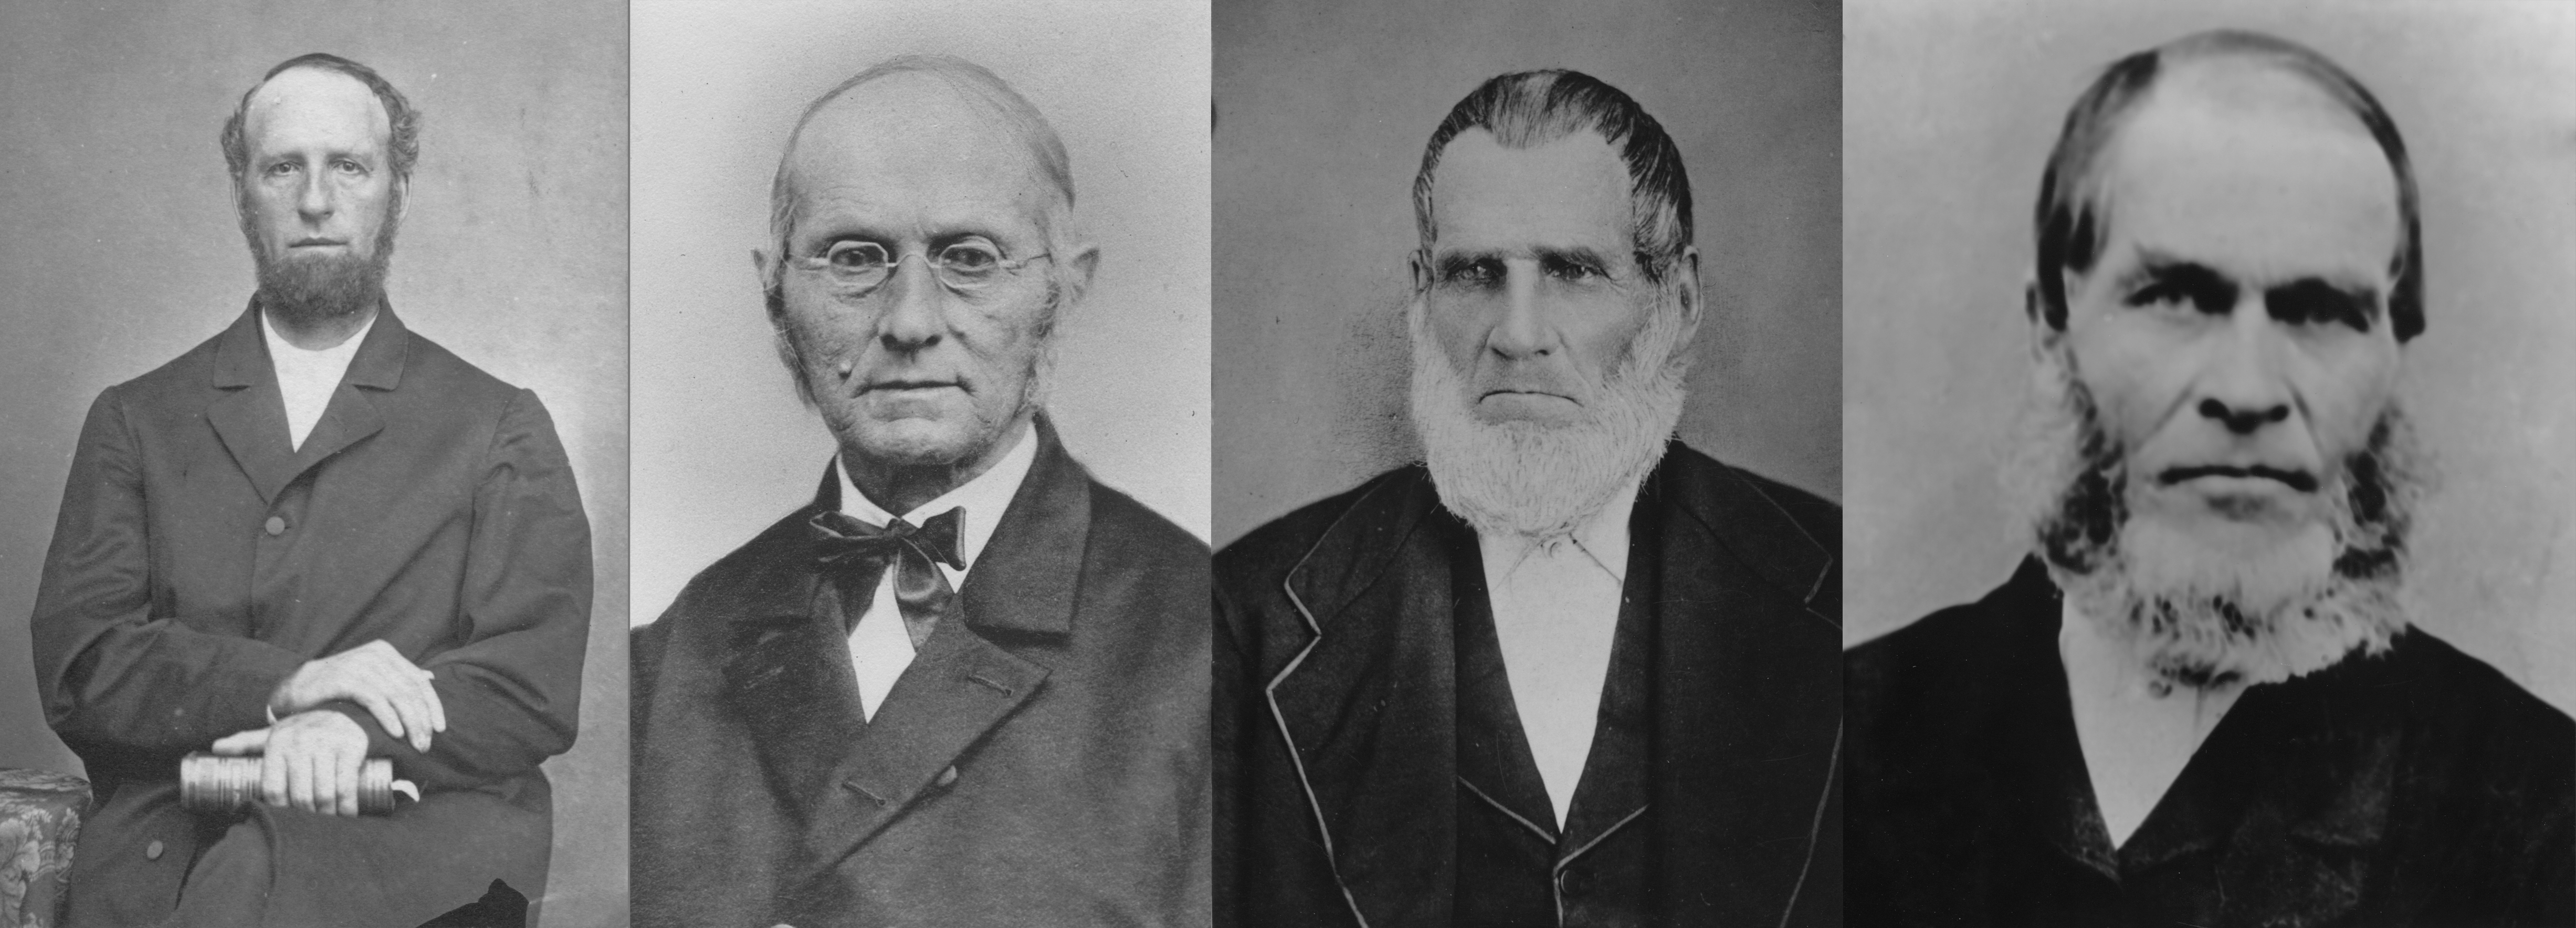
\includegraphics[width=1\linewidth]{images/james-white-joseph-bates-stephen-pierce-hiram-edson.jpg}
    \caption*{James White, Joseph Bates, Stephen Pierce, Hiram Edson}
    \label{fig:pioneers}
\end{figure}

\egwnogap{During this whole time I could not understand the reasoning of the brethren. My mind was locked, as it were, and I could not comprehend the meaning of the scriptures we were studying. This was one of the greatest sorrows of my life. \textbf{I was in this condition of mind until all \underline{the principal points of our faith} were made clear to our minds, in harmony with the word of God}. The brethren knew that when not in vision, I could not understand these matters, and they accepted as light direct from heaven the revelations given.}[SpTB02 57.1; 1904][https://egwwritings.org/read?panels=p417.291]

\egwnogap{For two or three years my mind continued to be locked to an understanding of the Scriptures. In the course of our labors, my husband and I visited Father Andrews, who was suffering intensely with inflammatory rheumatism. We prayed for him. I laid my hands on his head, and said, ‘Father Andrews, the Lord Jesus maketh thee whole.’ He was healed instantly. He got up, and walked about the room, praising God, and saying, ‘I never saw it on this wise before. Angels of God are in this room.’ The glory of the Lord was revealed. Light seemed to shine all through the house, and an angel’s hand was laid upon my head. From that time to this I have been able to understand the word of God.}[SpTB02 57.2; 1904][https://egwwritings.org/read?panels=p417.292]

\egwnogap{\textbf{What influence is it that would lead men at this stage of our history to work in an underhanded, powerful way \underline{to tear down the foundation of our faith},—the foundation that was laid at the beginning of our work by prayerful study of the word and by revelation? Upon \underline{this foundation} we have been building for \underline{the past fifty years}. Do you wonder that when I see the beginning of a work that would \underline{remove some of the pillars of our faith}, I have something to say? I must obey the command, ‘Meet it!’}}[SpTB02 58.1; 1904][https://egwwritings.org/read?panels=p417.295]

\egwnogap{I have the tenderest feelings toward Dr. Kellogg. For many years I have tried to hold fast to him. God’s word to me has always been, ‘You can help him.’ Sometimes I am awakened in the night, and, rising, I walk the room, praying: ‘O Lord, hold Dr. Kellogg fast. Do not let him go. Keep him steadfast. Anoint his eyes with the heavenly eyesalve, that he may see all things clearly.’ Night after night I have lain awake, studying how I could help him. Earnestly and often I have prayed that the Lord may not permit him to turn away from sanctifying truth. This is the burden that weighs me down,—the desire that he shall be kept from making mistakes that would hurt his soul and \textbf{injure the cause of present truth}. But for some time his actions have revealed that a strange spirit is controlling him. The Lord will take this matter in His own hands. I must bear the messages of warning that God gives me to bear, and then leave with the Lord the results. \textbf{I must now present the matter in all its bearings; for the people of God must not be despoiled}.}[SpTB02 58.2; 1904][https://egwwritings.org/read?panels=p417.296]

\egwnogap{\textbf{We are God’s commandment-keeping people. For the past fifty years every phase of heresy has been brought to bear upon us, to becloud our minds regarding the teaching of the word},\textbf{—especially concerning the ministration of Christ in the heavenly sanctuary, and the message of heaven for these last days, as given by the angels of the fourteenth chapter of Revelation}. \textbf{Messages of every order and kind have been urged upon Seventh-day Adventists, to take the place of the truth which, \underline{point by point}, has been sought out by prayerful study, and testified to by the miracle-working power of the Lord}. \textbf{But \underline{the way-marks} \underline{which have made us what we are}, \underline{are to be preserved}, and they \underline{will be preserved}, as God has signified through His word and the testimony of His Spirit}. \textbf{He calls upon us to \underline{hold firmly}, with the grip of faith, to \underline{the fundamental principles} that are \underline{based upon unquestionable authority}}.}[SpTB02 59.1; 1904][https://egwwritings.org/read?panels=p417.299]

There was a necessity to warn the church of the development of the enemy to uproot the foundation of our faith. There was a necessity to remind the church of what constitutes the true foundation of Seventh-day Adventist faith. It seems that Seventh-day Adventists, at that time, were forgetting \egwinline{the way the Lord has led us, and His teaching in our past history.}[LS 196.2; 1915][https://egwwritings.org/read?panels=p41.1083]

\egw{What influence is it that would lead men at this stage of our history to work in an underhanded, powerful way \textbf{to tear down the foundation of our faith},—the foundation that was laid \textbf{at the beginning of our work} by prayerful study of the word and by revelation? Upon \textbf{this foundation} we have been building for \textbf{the past fifty years}. Do you wonder that when I see the beginning of a work that would \textbf{remove some of the pillars of our faith}, I have something to say? I must obey the command, ‘\textbf{Meet it}!’}[SpTB02 58.1; 1904][https://egwwritings.org/read?panels=p417.295]

What was it that Sister White was commanded to meet?

\egwinline{About the time that ‘Living Temple’ was published} in the night season she received \egwinline{representations indicating that some danger was approaching,} and that she must \egwinline{prepare for it by writing out the things God has revealed} to her \egwinline{\textbf{regarding the foundation principles of our faith}.}

She was \egwinline{instructed by the heavenly messenger that some of the reasoning in the book, ‘Living Temple’, is unsound and that \textbf{this reasoning would lead astray} the minds of those who are not thoroughly established on \textbf{the foundation principles} of present truth.}

So, what was the actual problem with the book, “Living Temple”?

If you are a scholar, or an Adventist historian, or a theologian, or just a student of theology, before you give a straight answer and say that the problem was pantheism, we would like to point you back to the text. Sister White clearly addressed the core issue of the problem stating that the “Living Temple,” \egwinline{introduces that which is naught but speculation in \textbf{regard to the personality of God and where His presence is}.}

We do not deny the pantheistic problem of the book, but we want to divert attention from Kellogg’s error to the light God has given. There are two ways to approach Kellogg’s crisis. One is by addressing the pantheism, and another is to address \egwinline{\textbf{the personality of God} and \textbf{where His presence is}}. One way is to study the error, and the other way is to study the Truth. One way is to dissect the darkness and the other way is to drink from the fountain of the Truth. We choose the latter, and for this reason this book is set apart from hundreds of other books written on Kellogg’s crisis. The subject of this book is not pantheism, or any other error, but the truth and what God has revealed about His personality and where His presence is. This was the real issue of Kellogg’s publication. 

We believe it is a great danger to study and dissect the error because error leads to deception. The problem with deception is that we could be deceived obviously not knowing we are deceived! We firmly believe that Ellen White was the prophet of God and that she was receiving the Light from God \bible{who is light and in Him is no darkness at all}[1 John 1:5]. Therefore, we do not expect Sister White to explain the error in the book, “Living Temple”. Many were coming to her, asking her \egwinline{to explain the positions taken in ‘Living Temple.’} She replied, \egwinline{They are unexplainable}. Her objective was not to dissect the error but to shine the Truth on the \emcap{personality of God} and where His presence is. Thus, she was pointing back to the truths God founded the Seventh-day Adventist Church on. These truths have been constituting the foundation of our faith. These truths have been given to us in our early days. By diverting our attention from the personality of God to pantheism, we are losing an opportunity to remember \egwinline{\textbf{the way the Lord has led us}, and \textbf{His teaching} in our \textbf{past history}}. In this light, we express our concern over the Kellogg crisis and its pantheistic approach, because \egwinline{the track of truth lies close beside the track of error, and both tracks may seem to be one}; the solution to that is to be \egwinline{thoroughly established on \textbf{the foundation principles} of present truth}. Elsewhere, Sister White strongly established this principle.

\egw{Satan is by no means asleep; he is wide-awake and is playing the game of life for the souls of the people of God. He will come to them with flattery of all kinds, in the hope of leading them to swerve from their allegiance. \textbf{He desires to call their attention from the real issues to false theories}.}[Ms132-1903.42; 1904][https://egwwritings.org/read?panels=p9056.56]

So, let us focus our attention on the real issue instead of the false theories. 

% The Foundation of our Faith

\begin{titledpoem}
    \stanza{
        Pillars of truth, laid with care, \\
        By pioneers who sought in prayer. \\
        Principles firm, the Lord's design, \\
        A platform strong, for all time.
    }

    \stanza{
        Beware the subtle shifts that call, \\
        To change what should not change at all. \\
        Our identity, in these we find, \\
        God's revelations to mankind.
    }

    \stanza{
        Stand fast upon this solid ground, \\
        Where wisdom and God's light abound. \\
        Defend these truths with all your might, \\
        For in them shines eternal light.
    }
\end{titledpoem}